\documentclass[../main.tex]{subfiles}

\begin{document}

\subsection{Results for audiometric test functions}

The four test functions and six psychometric spread values we use add up to 24 total test function variants for the audiometric test function. To understand the broader performance patterns, we first illustrate a sample optimization run from the Metabolic+Sensory phenotype with $\beta=2$ in Fig.~\ref{fig:songexample}, comparing our contribution to prior methods. Under the linear-additive kernel, the model is overconfident in its ability to interpolate across the context dimension, and as a result oversmoothes the threshold and oversamples in one location. In contrast, both RBF models, while still taking some samples at the edges, spend more time exploring the interior of the threshold. Interestingly, the monotonic RBF model samples more at the edges in this specific example than the non-monotonic RBF model, again consistent with a pattern of greater boundary over-exploration being driven by model overconfidence. Finally, we see the RBF model perform similarly with and without the monotonicity constraint, something that we see in aggregate as well.

\begin{figure*}[!htb]
    \centering
    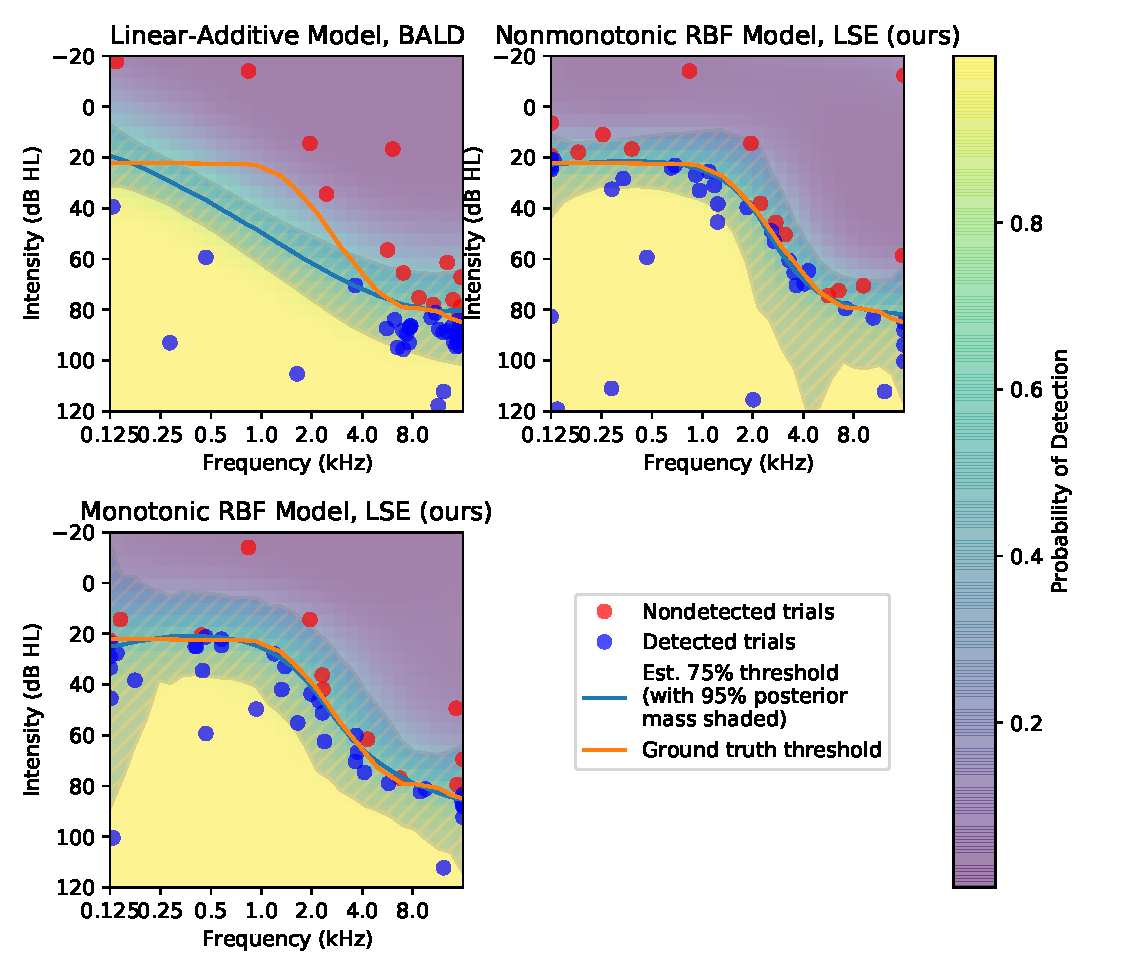
\includegraphics[width=\textwidth]{audio_lse_grids_fig.pdf}
    \caption{\textbf{Example of samples taken by three representative models on the Metabolic+Sensory test function after 50 trials with $\beta$=2}. All models begin with the same 5 trials generated from a Sobol sequence and then proceed according to their acquisition function (BALD in the case of the linear-additive model; LSE otherwise). Substantial boundary over-exploration is apparent in the linear-additive model, even with the addition of the previously-reported exploration heuristic. Both RBF models with the LSE objective sample consistently at putative threshold locations and produce good mean threshold estimates after only 50 trials.}
    \label{fig:songexample}
\end{figure*}

Next, we turn to the aggregate performance curves in Fig.~\ref{fig:songsims}. In the aggregate data, we see that the RBF kernel models we introduced consistently outperform the previously-reported linear-additive kernel models, for both threshold estimation and estimation of the full surface. In addition, we see the LSE acquisition function we introduced performed best for estimating the threshold, in the sense that it both reduced error the fastest and achieved the lowest error (occasionally tied with BALV/BALD) after 150 trials. This confirms the benefits of an acquisition function explicitly designed to target where the threshold is likely to be rather than sampling to reduce global uncertainty: in some cases LSE achieves the same error in well under 50 trials that BALD achieves in 150 trials. This comes with a tradeoff against estimating the full surface which the LSETS acquisition objective we introduced mitigates somewhat. Importantly, the improvements provided by our contributions can be seen even in this setting, where test functions are generated in accordance with the additive structure in the linear-additive model.

\begin{figure*}[!htb]
    \centering
    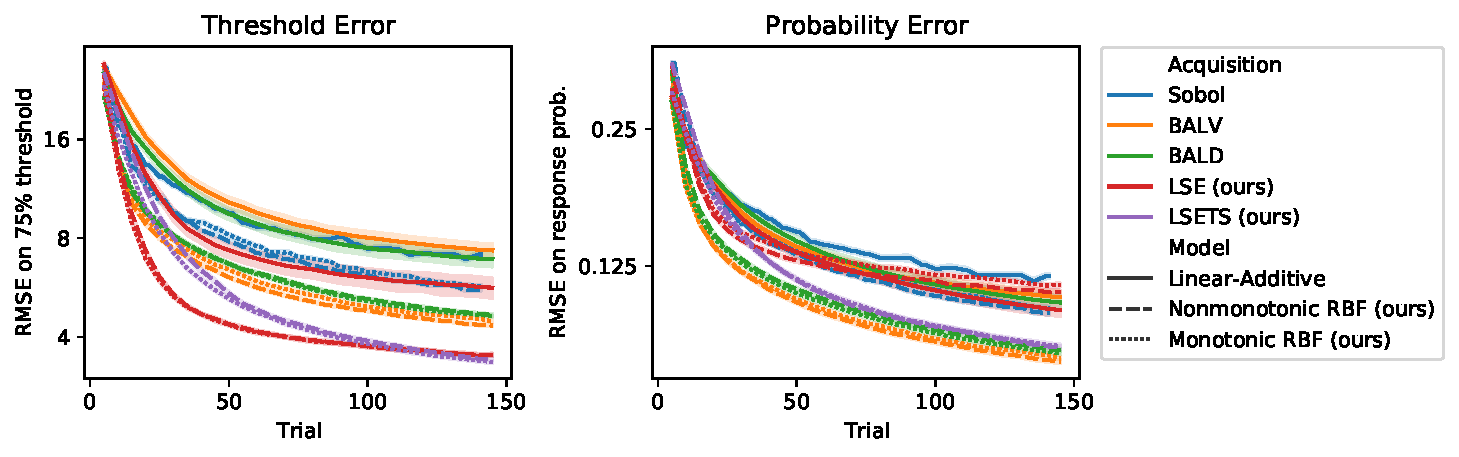
\includegraphics[width=1.1\textwidth]{audiometric_perf.pdf}
    \caption{\textbf{Audiometric test function performance}. \emph{Left}: For threshold estimation, LSE consistently the best objective, consistent with its explicit targeting of putative threshold locations, independent of model. \emph{Right}: For estimating the full posterior, BALV appears superior in this setting, followed by all the other objectives excluding LSE, whose focus on the threshold location leads to undersampling of the rest of the surface. In both evaluations, the monotonic and nonmonotonic RBF models are far superior to the linear-additive model, whose average performance is poor overall. Finally, the benefit of monotonicity seems minor at best over the nonmonotonic model. Shaded intervals are a 0.95 confidence interval over simulations. Note the log-scale on the y-axis.}
    \label{fig:songsims}
\end{figure*}

Finally, we report the final performance for all individual audiometric test functions in terms of error probability in Fig.~\ref{fig:song-p} and threshold in Fig.~\ref{fig:song-thresh}. In this breakout we see one outlier, the older-normal phenotype, where the linear-additive kernel model outperforms the RBF models (though even here, the LSE objective is superior to BALD and BALV for threshold estimation). We discuss this discrepancy below.

Surprisingly, we did not see a substantial benefit from the monotonic model in our evaluations. While numerically it seems like the monotonic model outperforms the unconstrained RBF model at very small numbers of trials (under about 25), the effect washes out later in the experiment. We suspect this is because for all the test functions we evaluated, the monotonicity property is relatively easy to learn from data: there are large areas of the space where the response probability is either 0 or 1. We suspect that the underperformance of the monotonic model, when it happens, is due to reduced exploration driven by increased confidence, similarly to the linear-additive model. Nonetheless, we think monotonicity is an important addition to the model for theoretical soundness and interpretability by practitioners, as discussed earlier.

\begin{figure*}[!htb]
    \centering
    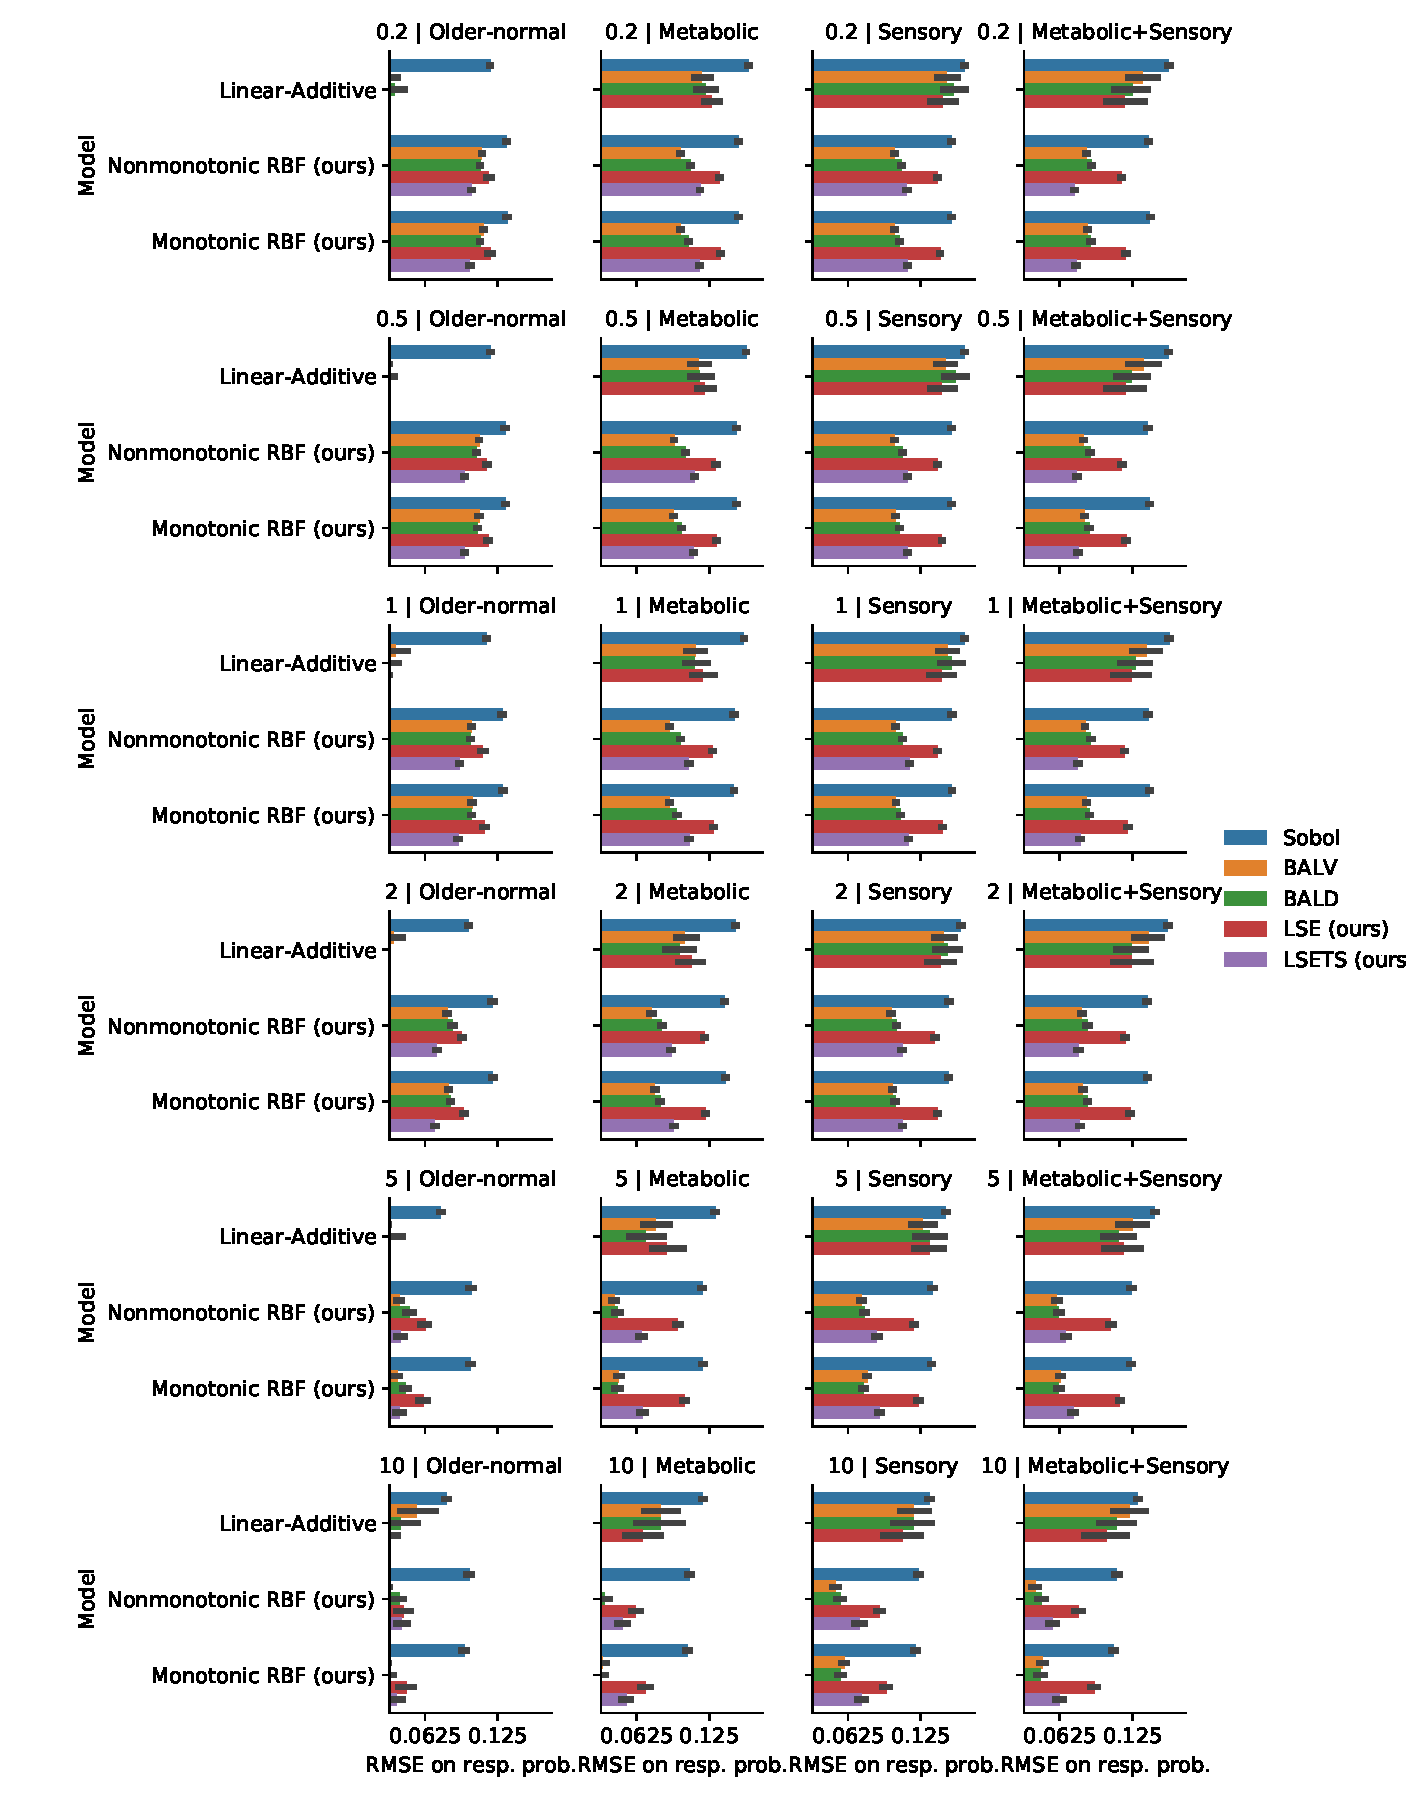
\includegraphics[height=\textheight]{audio_p_final.pdf}
    \caption{\textbf{Audiometric test function final probability performance}. The overall pattern is heterogenous, but we highlight a few points: first, BALV and BALD are superior to LSE and LSETS when it comes to estimating the full psychometric function, consistent with the latter's focus on estimating the threshold only. Second, the RBF models outperform the linear-additive model, except for the older-normal phenotype. Error bars are a 0.95 confidence interval over simulations. Note the log scale on the x-axis. }
    \label{fig:song-p}
\end{figure*}

\begin{figure*}[!htb]
    \centering
    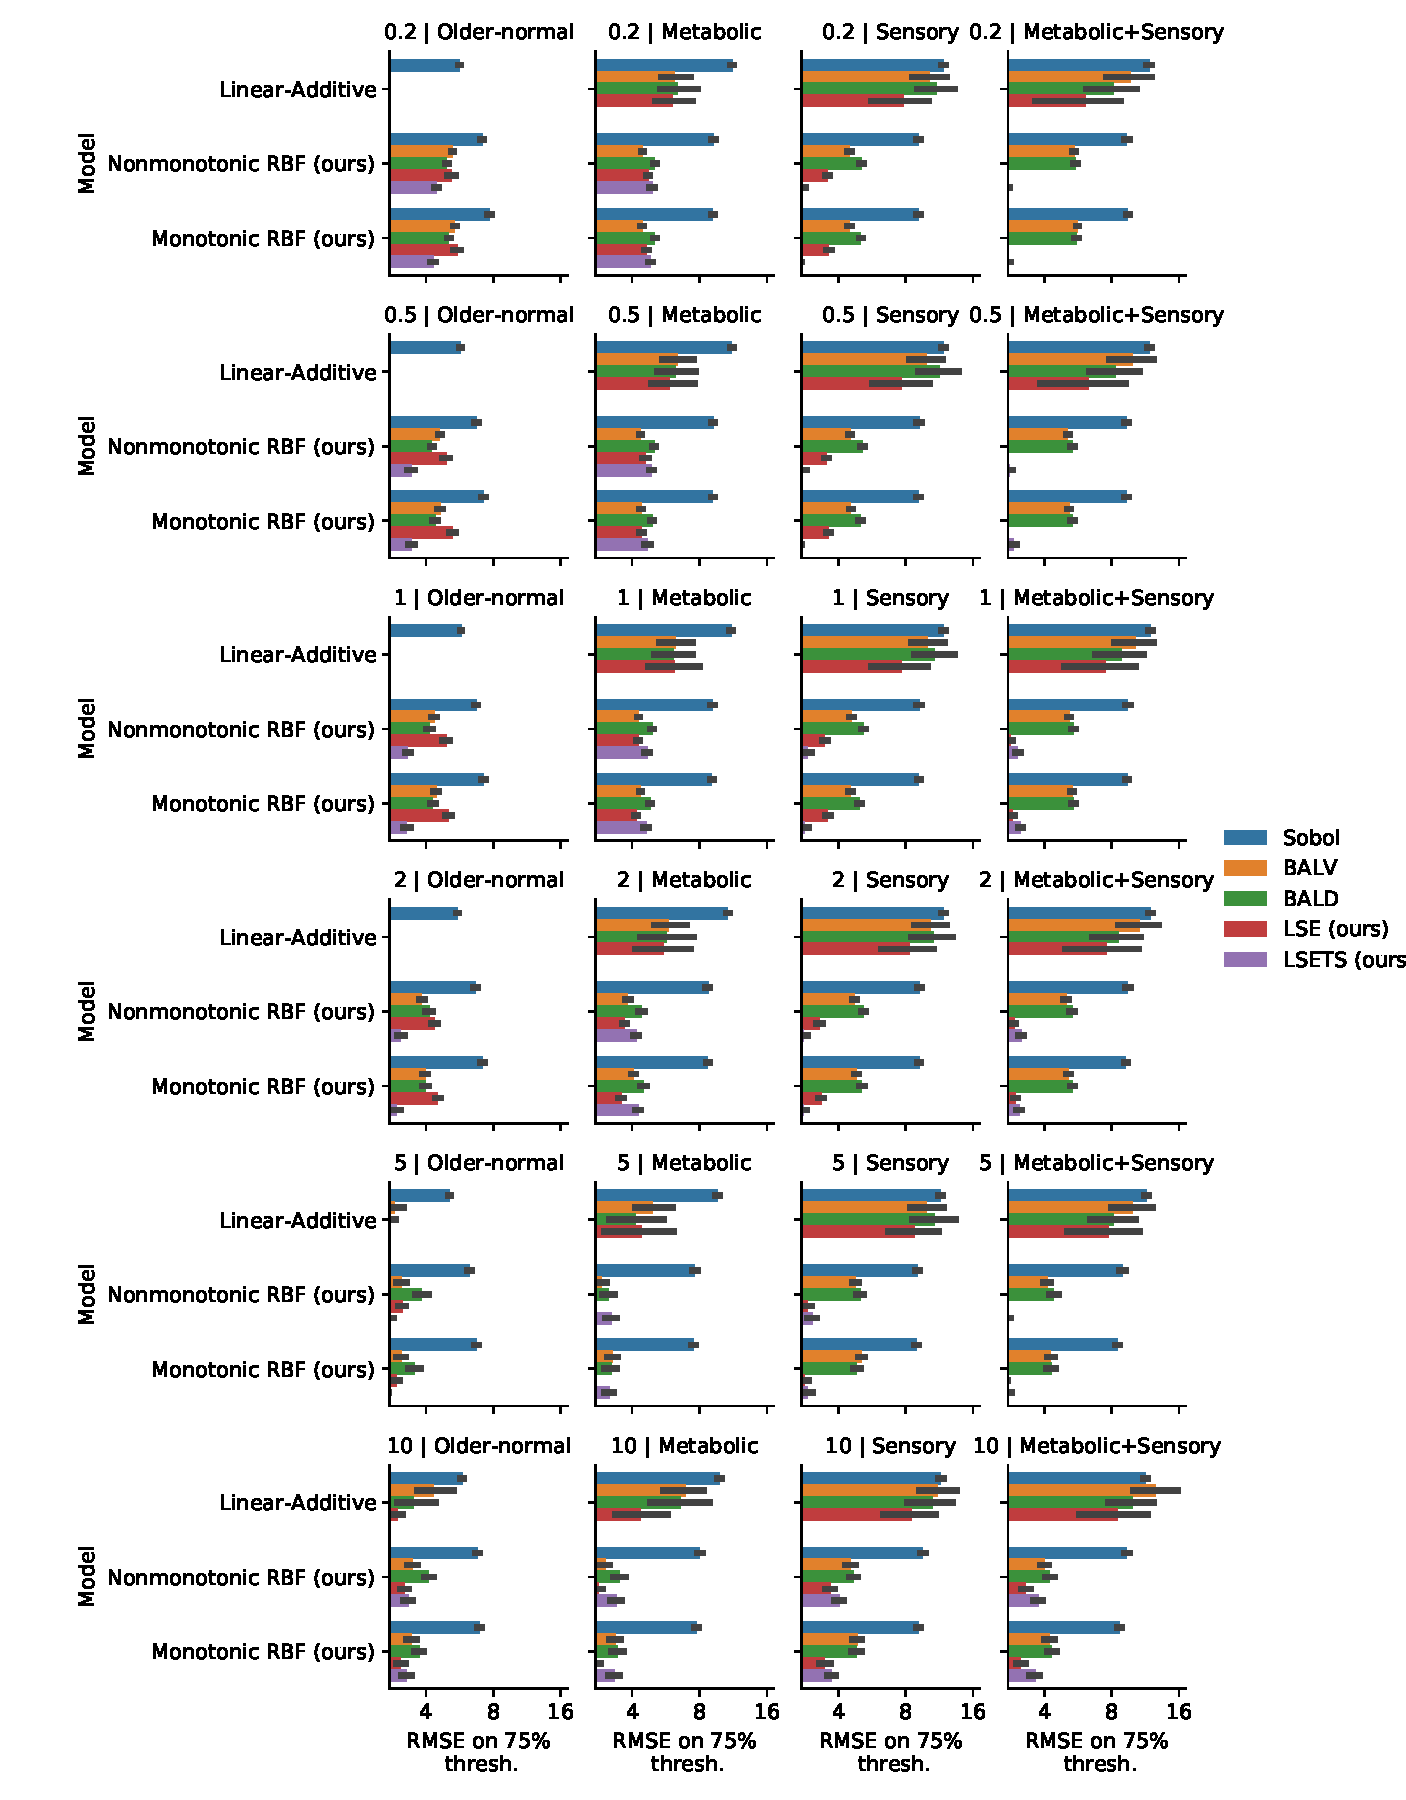
\includegraphics[height=\textheight]{audio_thresh_final.pdf}
    \caption{\textbf{Audiometric test function final threshold performance}. The overall pattern is heterogenous, but we highlight a few points: first, the LSE and LSETS objectives consistently perform well for threshold estimation, consistent with their focus on threshold estimation (though sometimes BALD and BALV do well also). Second, the RBF models outperform the linear-additive model, except for the older-normal phenotpye. Errorbars are a 0.95 confidence interval over simulations. Note the log scale on the x-axis}
    \label{fig:song-thresh}
\end{figure*}

\subsection{Results for novel test functions}

\subsubsection{Novel detection test function}
As with the audiometric test functions, we begin with illustrative examples. A run from the novel detection test function is shown in Fig.~\ref{fig:detection_example}, where we see the same clustered sampling behavior for the linear-additive model seen in the audiometric example. The overall threshold shape appears correct, but the model is expectedly inaccurate in areas where it undersampled. The RBF kernel model performs well regardless of the monotonicity constraint, and while there may appear to be a slight difference in threshold accuracy in the figure, it is not seen in aggregate data. This aggregate data is seen in Fig.~\ref{fig:detection_perf}, where the pattern is very similar to the audiometric setting: the RBF models far outperform the linear-additive model, and LSE outperforms the other objectives for threshold estimation while expectedly falling short in error over the probability surface. In contrast to the audiometric setting, the LSETS acquisition function does not provide a middle ground, patterning with the global objectives in threshold error while failing to match them in probability error.

\begin{figure*}[!htb]
    \centering
    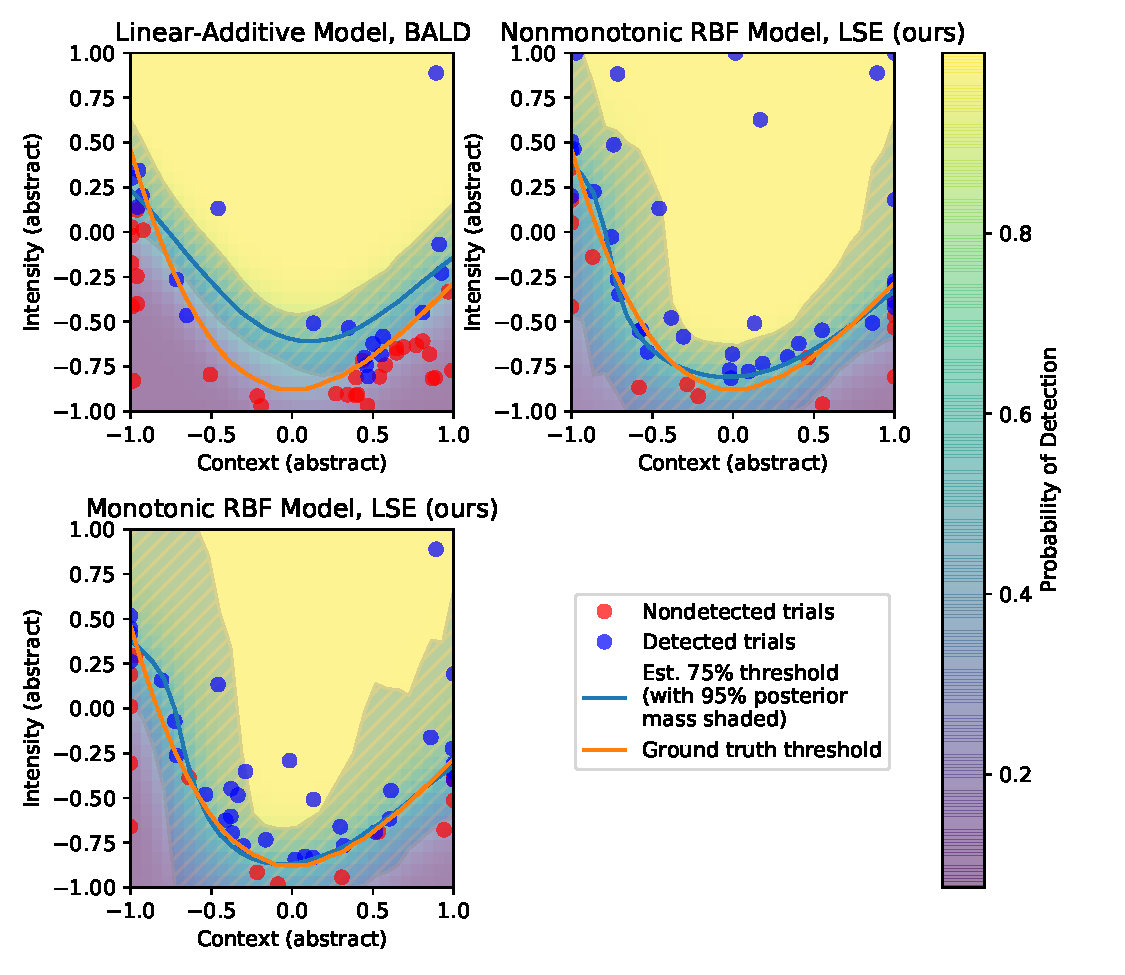
\includegraphics[width=\textwidth]{detection_lse_grids_fig.pdf}
    \caption{\textbf{Example of samples taken by three representative models on the novel detection test function after 50 trials}. All models begin with the same 5 trials generated from a Sobol sequence and then proceed according to their acquisition function (BALD in the case of the linear-additive model; LSE otherwise). The linear-additive model oversamples the right side of the space, likely due to over-confidence driven by the additive structure. The final estimate does not overlap the true threshold on the left of the plot. Both RBF models with the LSE objective produce good mean threshold estimates. Note that the nonmonotonic model takes multiple samples at the upper and lower boundaries of the space, whereas the monotonic model does not because the monotonicity constraint makes it highly unlikely that the threshold is located there.}
    \label{fig:detection_example}
\end{figure*}

\begin{figure*}[!htb]
    \centering
    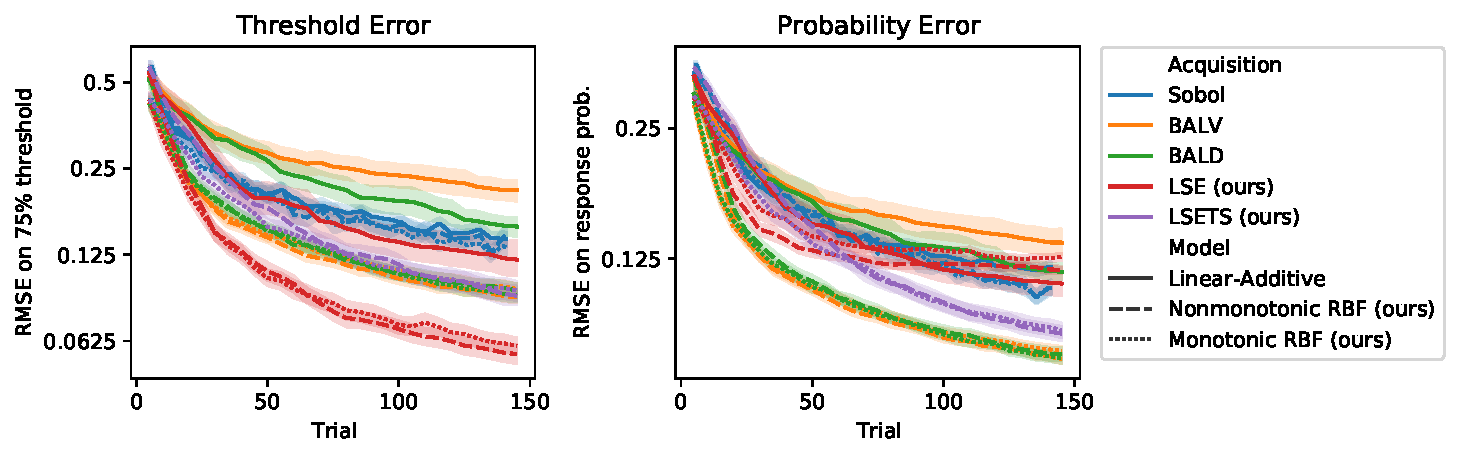
\includegraphics[width=\textwidth]{det_perf.pdf}
    \caption{\textbf{Novel detection test function performance}. LSE is competitive in terms of error in both threshold (\emph{left}) and probability (\emph{right}), followed by BALV/BALD and LSETS. For very small numbers of trials, the linear additive model's strong priors allow it to outperform the more flexible models, but with more data the restrictive assumptions hold it back. The monotonic model generally fails to outperform the nonmonotonic one. Shaded intervals are a 0.95 confidence interval over simulations. }
    \label{fig:detection_perf}
\end{figure*}

\subsubsection{Novel discrimination test function}
A run on the novel discrimination test function is shown for our three representative models in Fig.~\ref{fig:discrimination_example}. This is the hardest test function we explored, in that its domain only covers probabilities above 0.5. Here the linear-additive model with BALD breaks down completely and fails to recover any threshold, spending its entire time sampling stimuli at the edges of the space. In contrast, both RBF models with LSE still estimate reasonable thresholds in this setting. While we see apparent numerical benefits for the monotonic model, these again fail to be borne out in aggregate results, which are shown in Fig.~\ref{fig:detection_perf}. In aggregate, the RBF models we introduce again outperform the linear-additive model, and while the monotonicity constraint provides performance benefits for some acquisition functions, it does not do so for the best-performing ones. When it comes to acquisition, the LSE objective we introduced once more performs best for threshold estimation, though the gap is smaller than in the easier cases. For estimating the full probability surface, LSE surprisingly patterns with the global objectives in this problem.

\begin{figure*}[!htb]
    \centering
    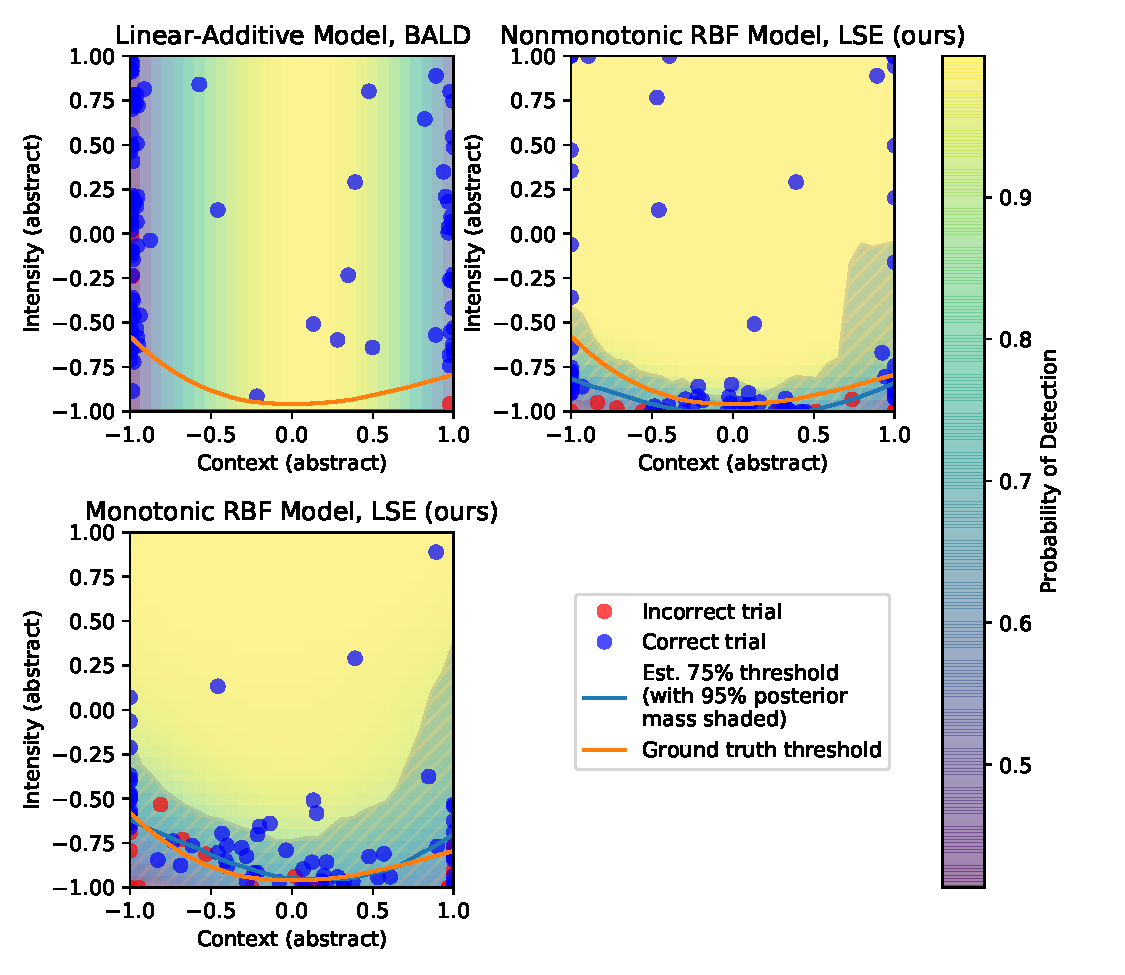
\includegraphics[width=\textwidth]{discrimination_lse_grids_fig.pdf}
    \caption{\textbf{Example of samples taken by three representative models on the novel discrimination test function after 100 trials}. All models begin with the same 5 trials generated from a Sobol sequence and then proceed according to their acquisition function (BALD in the case of the linear-additive model; LSE otherwise). We used 100 rather than 50 example trials here because the test function is substantially more difficult than the others. The linear-additive model with BALD fails completely on this task: after observing a few correct trials (consistent with the whole space generating probabilities above 0.5), the model is over-confident over the interior of the space and solely samples at the edges. Both RBF models perform acceptably, though in this case the monotonic model spends fewer trials sampling the upper and side edges (where the threshold is unlikely to be under the monotonicity assumption), and achieves a more accurate mean estimate. This pattern was not consistent on average over replications, however. }
    \label{fig:discrimination_example}
\end{figure*}

\begin{figure*}[!htb]
    \centering
    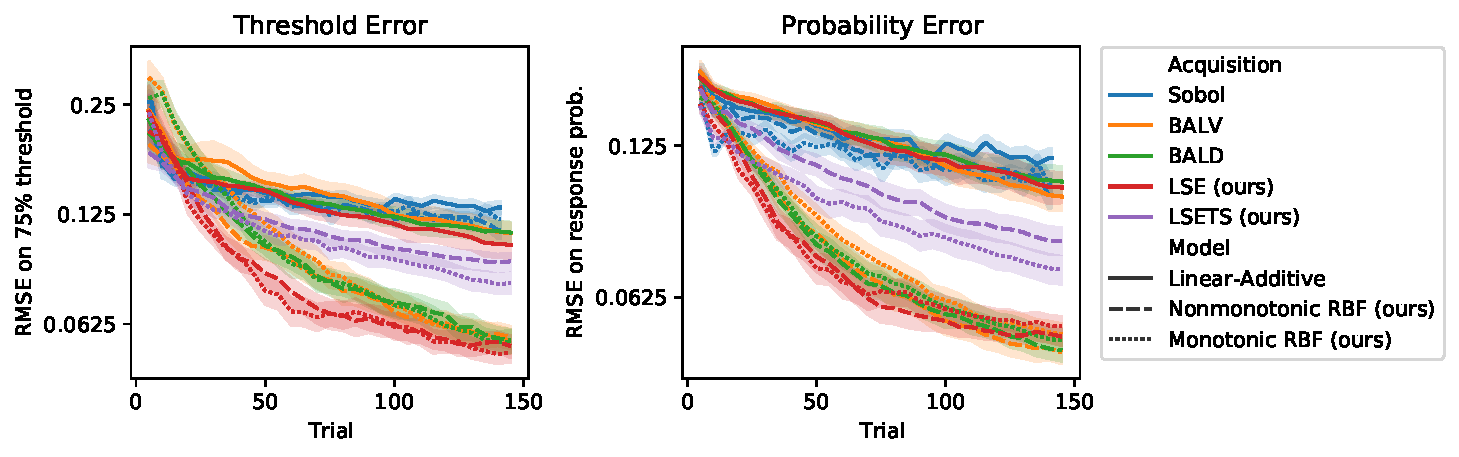
\includegraphics[width=\textwidth]{disc_perf.pdf}
    \caption{\textbf{Novel discrimination test function performance}. LSE performs best in terms of error in threshold (\emph{left}) whereas the global acquisition objectives BALD and BALV both perform the best in terms of error in probability  (\emph{right}). LSETS shows competitive (but not winning) performance in both. The full-RBF models consistently outperform the linear-additive model, but the monotonic model largely fails to beat the nonmonotonic one. Shaded intervals are a 0.95 confidence interval over simulations. }
    \label{fig:discrimination_perf}
\end{figure*}

\end{document}
